\chapterimage{./Images/head2.jpg} % Chapter heading image
\chapter{Diodes contd. - Chapter 4 of the Textbook}

\begin{example}
    \begin{figure}[H]
        \centering
        \begin{circuitikz}
            \draw
            (0,0) to[diode] (0,-2)
            (0,0) node[anchor=east] {5V}
            (0,-2) to[ground] (0,-4)
            (0,-2) node[anchor=west] {};
        \end{circuitikz}
        \caption{Diode}
    \end{figure}


    \[i = ? \quad
        v = ? \]

    Case I: Diode is forward biased
    \begin{figure}[H]
        \centering
        \begin{circuitikz}
            \draw
            (0,0) node[anchor=east] {5V}
            (0,0) to[ground] (0,-4)
            (0,0) node[anchor=west] {};
        \end{circuitikz}
        \caption{Diode}
    \end{figure}
    \[V = 5V \quad i = 0 \]

    Case II: Diode is reverse biased
    \begin{figure}[H]
        \centering
        \begin{circuitikz}
            \draw
            (0,0) to[short, -o] (0,-2)
            (0,0) node[anchor=east] {5V}
            (0,-2) to[short, o-] (0,-4)
            (0,-2) node[anchor=west] {};
        \end{circuitikz}
        \caption{Diode}
    \end{figure}
    \[V = 0V \quad i = V/R = 5A \]
\end{example}

\section{Rectifier Circuits}
\begin{definition}
    [Rectifier]
    \begin{itemize}
        \item Converts AC to DC
        \item Uses diodes
    \end{itemize}
\end{definition}

\begin{figure}
    \centering
    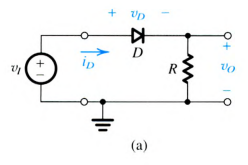
\includegraphics[scale=1]{./LECTURE_2/rectifier.png}
    \caption{Rectifier}
\end{figure}

\begin{example}
    [Half-wave Rectifier]
    \begin{figure}[H]
        \centering
        \begin{circuitikz}
            \draw
            (0,0) to[sV, l=$V_{in}$] (0,4)
            (0,4) to[diode] (4,4)
            (4,4) to[R, l=$R$] (4,0)
            (4,0) to[short, -o] (0,0)
            (4,0) node[anchor=north] {GND};
        \end{circuitikz}
        \caption{Half-wave Rectifier}
    \end{figure}
    A voltage with the following waveform is applied to the input of the half-wave rectifier will change in the following way:
    \begin{figure}[H]
        \centering
        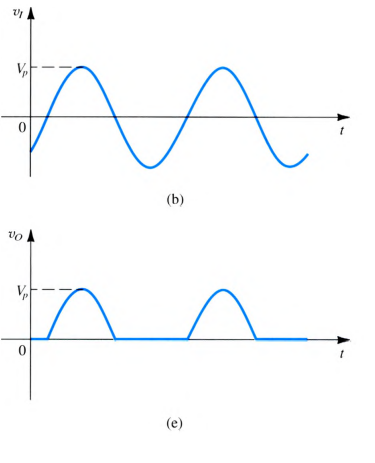
\includegraphics[scale=1]{./LECTURE_2/waveform.png}
        \caption{Waveform}
    \end{figure}
    Because when the input voltage is negative, the diode is reverse biased and the output voltage is 0V. But when the input voltage is positive, the diode is forward biased and the output voltage is the same as the input voltage.
\end{example}

\begin{remark}
    When solving a circuit with multiple diodes, it is important to consider the state possibility of each diode. For example, with 2 diodes, consider the following states:
    \begin{itemize}
        \item Both diodes are forward biased
        \item Both diodes are reverse biased
        \item The first diode is forward biased and the other is reverse biased
        \item The second diode is forward biased and the other is open
    \end{itemize}
\end{remark}

\begin{example}
    [Two Diode Circuit]
    \begin{figure}[H]
        \centering
        \begin{circuitikz}
            \draw
            (0,0) to[R, l=$5k\Omega$] (0,-2)
            (0,-2) to[diode, l = $D_2$] (0,-4)
            (0,-4) -- (-2,-4)
            (-2,-6) to[diode, l = $D_1$] (-2,-4)
            (0,-4) to[R, l = $10k\Omega$] (0,-6);
            \node at (0,-6) [anchor=east] {-10V};
        \end{circuitikz}
        \caption{Two Diode Circuit}
    \end{figure}
    Show that $D1$ is forward biased and $D2$ is reverse biased. \textit{Hint: Use nodal analysis.}
\end{example}
\section{Diode Logic}

\begin{example}
    [OR Gate]

    \begin{figure}
        \centering
        \begin{circuitikz}
            \draw
            (0,0) to[diode, l=$V_A$] (2,0)
            (2,0) -- (2,-2)
            (0,-2) to[diode, l=$V_B$] (2,-2)
            (2, -2) to[short, -o, l=$v_o$] (4, -2)
            (2,-2) to[R, l=$R$] (2,-4);
        \end{circuitikz}
        \caption{Diode Logic}

    \end{figure}
    Show with a truth table that this is an OR gate.

    Two conflicting diodes are both on, but two vs. one diode will turn the one off. The output voltage is the same as the input voltage.
\end{example}